\section{Old version of two-replica proofs}
We have seen that replica selection flexibilities can render embeddings computationally hard.
We will now provide a more detailed look at this hardness result
and explore the minimal requirements for rendering replica selection hard.
In particular, we will show that already two replicas for each chunk type are sufficient to
introduce intractability.

Across the next sections, we use the following notation:

\begin{enumerate}
  \item $n := |X|$ (remember that $|X| = |Y| = |Z|$)
  \item $e$ -- an element of the universe ($e \in X \cup Y \cup Z$)
  \item $T$ -- set of triples
  \item $t = |T|$
  \item $T_e$ -- set of triples that contain element $e$
  \item $\deg(e) := |T_e|$
  \item $\lbrace e_X(\tau), e_Y(\tau), e_Z(\tau) \rbrace$ -- elements of triple $t$
  \item $V$ -- set of nodes to be spawned in embedding instance
\end{enumerate}

\subsection{Two Replicas without Bandwidth Constraints}

We now show that the 2-replica selection problem is even NP-hard
without capacity constraints.  In particular, we consider the problem
variant~$\RS(2)+\MA(4)+\FP$ with at most two replicas of each chunk type and assignment factor
four. There are no capacity constraints on links.

\textbf{Construction.}

Let's take any instance~$I_{\TDPM}$ of~$\TDM$ and create a~$\RS(2)+\MA(4)+\FP$
instance~$I_{\VCEMB}$ as follows.

\paragraph{Chunks}

We construct three types of chunks. The first type corresponds to covers of elements by triples, with two replicas each. The other two types are chunk types with one replica only, therefore called \emph{unique}. We construct two types of unique chunks, distinguished by a different role in the construction. For unique chunks we simply annotate the chunk type with chunk replica.
Thus, the constructed instance uses at most two replicas of each chunk type.

\begin{enumerate}
  \item For each triple $\tau \in T$, we construct $3$ chunk types, with two replicas each. We construct different chunk types for each triple $\tau$, which 
  contain element $e$. We refer to those replicas by $ch_1(e, \tau)$ and $ch_2(e, \tau)$.
  \item We construct~$n$ additional chunk types named
  ~$u_1, \ldots, u_n$, with one replica each.
  \item For each element~$e\in X\cup Y\cup Z$,
  we construct additional~$3\cdot(\deg(e) - 1)$ chunks, with one replica each.
  We call this set~$\UniqueE$.
\end{enumerate}

\paragraph{Tree}

We construct the following tree.

\begin{figure}[t]
  \centering
  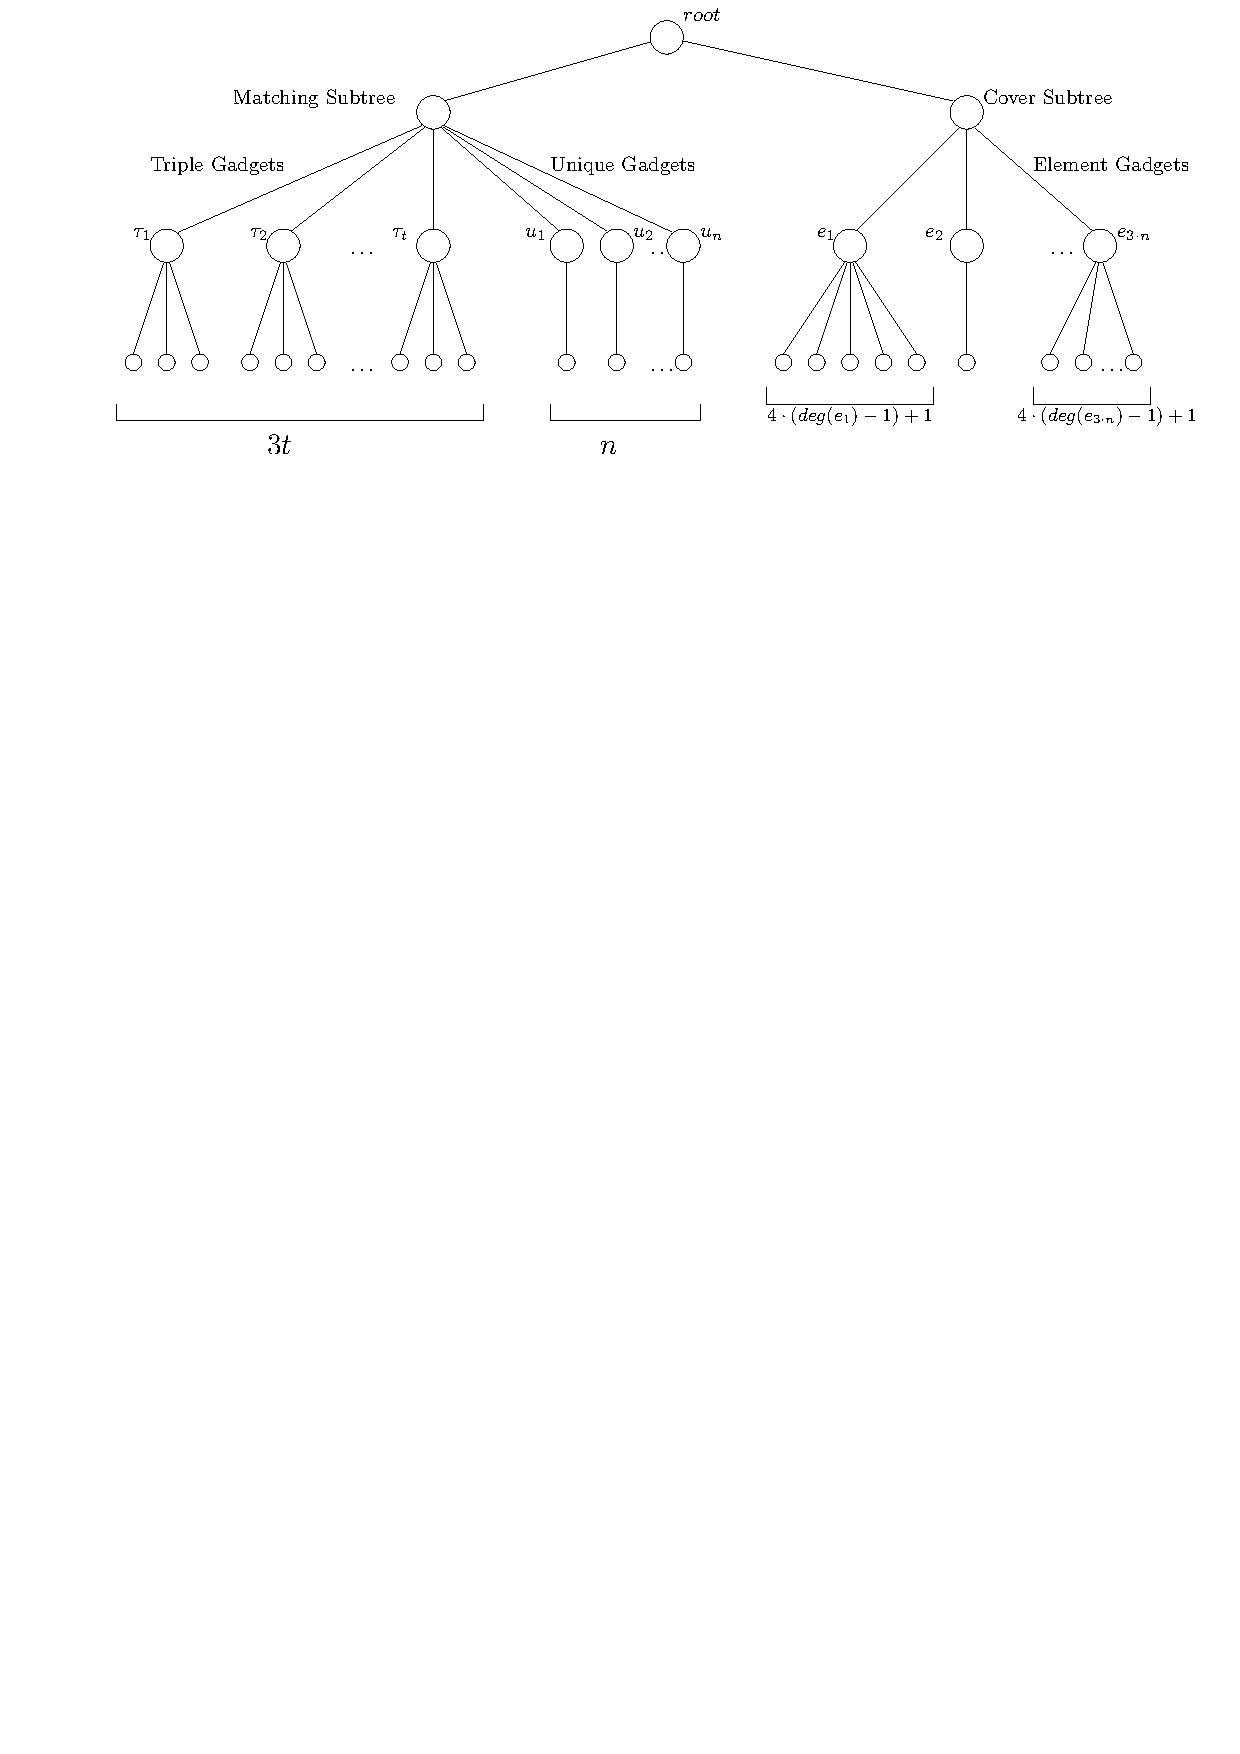
\includegraphics[width=0.99\columnwidth]{reduction/overview.pdf}
  \vspace{-1em}
  \caption{Overview of the substrate network}
  \vspace{-1em}
\end{figure}


\begin{enumerate}
  \item The physical network consists of two subtrees connected to the
  root: A {\MatchSubtree} and a {\CoverSubtree}. The
  {\MatchSubtree} consists of $|T|$ {\TripleGadgets}, one per each triple $t\in T$ and $n$
  {\UnqGadgets}. The {\CoverSubtree} consist of~$n$ {\ElGadgets}, one for each element $e\in X\cup Y\cup Z$.
  \item {\TripleGadget} consists of four vertices: three leaves and the root of the gadget.
  \item {\UnqGadget} consists of two vertices: the leaf and the root of the gadget. Note that we construct
  nodes not only to keep the tree balanced, but also to keep leaves of
  {\UnqGadgets} far from leaves of other \UnqGadgets.
  \item {\ElGadget} of element $e$ has a structure that depends on the number of triples that cover $e$. The {\ElGadget} consists of the
  root, and~$4\cdot(\deg(e)-1)+1$ leaves.
\end{enumerate}

\paragraph{Chunk Placement}
The chunks are placed as follows:
\begin{enumerate}
  \item \emph{Chunks in matching subtree:} In {\TripleGadget} of triple $\tau$ we put
  three replicas:
 ~$ch_1(e_X(\tau), \tau), ch_1(e_Y(\tau), \tau), ch_1(e_Z(\tau), \tau)$, one per each leaf.
  \item \emph{Chunks in unique subtree:} We place replicas
 ~$u_1,\ldots, u_n$ at the leaves of \UnqGadgets.
 \item \emph{Chunks in element gadget:} In leaves {\ElGadget} of element $e$ we put replicas $ch_2(\tau, e)$ for each $\tau \in T_e$. Additionally, we put replicas $\UniqueE$.
\end{enumerate}

\paragraph{Other properties of the instance}
\begin{enumerate}
  \item \emph{Multiple assignment:} We set the assignment factor (number of processed
  chunks by each node) to four.
  \item \emph{Number of nodes:} We allow to spawn
 ~$\numNodes := n + \sum_{e}(\deg(e)-1)$ nodes.
  \item \emph{Threshold:} We set the following threshold for cost of a solution to be feasible.
 ~$\Thr := 8\cdot n + 6\cdot\sum_{e}(\deg(e)-1)$
\end{enumerate}


\textbf{Reduction.}  We can make the following observations.

\begin{obs}
  The construction fulfills the following properties:
  \begin{enumerate}
    \item There is exactly one replica of each chunk type (except\hspace{1mm} $\UniqueE$ for each edge $e$) in the
    \MatchSubtree.

    \item There is exactly one replica of each chunk type in the
    \CoverSubtree.

    \item There are at most two replicas of each chunk type in the
    substrate network.
  \end{enumerate}
\end{obs}

For the reduction we proceed as follows:
\begin{enumerate}
  \item Let's take any instance $I_{\TDM}$ of $\TDM$ and produce an instance $I$ as described in the construction section.
  \item Let's take any feasible solution $S_{\TDM}$ to $I_{\TDM}$ and place $n$ (remember that~$n=|X|=|Y|=|Z|$) nodes in the following way: for each triple $r$ chosen in $S_{\TDM}$ solution, we select an arbitrary leaf of the Triple Gadget corresponding to $r$ and place a node there.
  We
  match each such node to three chunks that are put in its
  {\TripleGadget} (it is co-located with one of the chunks), and we match it to an
  arbitrary unmatched chunk in any \UnqGadget.
  \item We put~$\deg(e)-1$ nodes in each \emph{Element Gadget}. We match all
  remaining chunks from this \emph{Element Gadget} to those nodes in an
  arbitrary way.
  \item This solution has cost~$\leq \Thr$ (easy to see by summing up the
  costs of transporting chunks to each node).
  \item The feasibility of the constructed solution follows from the
  fact that each chunk type was processed; each node processes four
  chunks.
\end{enumerate}

\textbf{Proof of correctness of the reduction.}

Before we start the reduction, let us introduce two functions that will help us show that certain node placements are infeasible, as their cost exceeds the threshold.
  For each $u \in \{ 1, \ldots, t-1 \}$ let us define
 ~$\CostEstimOne(u) = u \cdot 12 + (\tau-u)\cdot 4 + (4\cdot n -
  n - 4\cdot u - (\tau-u))\cdot 2$, and 
$\CostEstimTwo(u) = 4\cdot \tau + (4\cdot
n - n - \tau)\cdot 2$, where $\tau$ is the number of triples and $n = |X| = |Y| = |Z|$ in a given instance of $\TDM$.
We use the function $\CostEstimOne(u)$ in Lemma~\ref{th:no-unique} to show that no node spawned in the Unique Subtree: the $\CostEstimOne(u)$ is the lower-bound on the total cost of the solution, assumming that $u$ nodes spawned in the Unique Subtree.
By Lemma~\ref{lem:cost-estims}, for non-zero $u$ the cost lower-bound already exceeds the threshold.
and we use the function $\CostEstimTwo$ in Lemma~\ref{th:np-balance} to show that exactly $n$ nodes spawned in the Matching Subtree. \maciek{After fixing the proof np-balance, write what $u$ corresponds to}

\begin{lemma}
  For each $u \in \{ 1, \ldots, t-1 \}$ we have that $\CostEstimOne(u) > \Thr$ and
  $\CostEstimTwo(u) > \Thr$.
  \label{lem:cost-estims}
\end{lemma}

\begin{proof}
  We have that $\CostEstimOne(u+1) \geq \CostEstimOne(u)$ and $\CostEstimTwo(u+1) \geq \CostEstimTwo(u)$ , for
 ~$1\leq u \leq t-1$. It is easy to verify that $\CostEstimOne(1) > \Thr$ and $\CostEstimTwo(1) > \Thr$.
\end{proof}

\begin{lemma}
  Take any feasible solution~$\Solution$ to the instance~$I$ of
 ~$\RS(2)+\MA(4)+\FP$ (as constructed above). If the cost of
 ~$\Solution$ is at most~$\Thr$, then no node is spawned in the Unique
  Subtree.
  \label{th:no-unique}
\end{lemma}

\begin{proof}
  For the sake of contradiction, let us assume a feasible solution
 ~$\Solution$ with at least one node spawned in {\UnqSubtree}. We show
  that in this case, the cost of solution~$\Solution$ is greater than
 ~$\Thr$. Let $\ell$ be the number of nodes spawned in the {\UnqSubtree}. We know
  that~$1 \leq \ell \leq |T|$.  In~$\Solution$ we have exactly
 ~$4 \cdot \numNodes$ chunk transportations, incurring cost
 ~$0, 2, 4$ or~$6$ (the tree has an edge-height of~$3$). At most
 ~$\numNodes$ transportations are of cost~$0$. Note that the leaves of the
  {\UnqSubtree} are separated from other leaves of the tree by at
  least~$4$ edges.  The cost of chunk transportation to nodes
 ~$v \in \SpawnedUnqSubtree$ is at least~$12$. The chunks in
  {\UnqSubtree} are unique, therefore the solution transports~$|T| - \ell$
  chunks to nodes outside the \UnqSubtree, incurring cost~$4$ for each
  chunk.
  Therefore $\CostSol \geq \CostEstimOne(\ell)$, and by Lemma \ref{lem:cost-estims}
  we conclude that $\CostSol > \Thr$.
\end{proof}



\begin{lemma}
  Given any feasible solution~$\Solution$ to a given instance~$I$ of
 ~$\RS(2)+\MA(4)+\FP$ (as constructed above). If the cost of
 ~$\Solution$ is at most~$\Thr$, then exactly~$n$ nodes are spawned in the
  \MatchSubtree.
  \label{th:np-balance}
\end{lemma}
\begin{proof}
    \maciek{This proof requires revision}
  Let~$\ell$ be the number of nodes spawned in
  {\MatchSubtree}.  Let us assume the contrary, namely that
 ~$\ell \neq n$.  First, we use
  Theorem~\ref{th:no-unique} to restrict the placement of nodes in
  \UnqSubtree. Then we consider two cases:
  \begin{enumerate}
    
    \item~\textbf{Case $\ell \leq n$:} There are at least
   ~$u := 4 \cdot (n-\ell)$ chunks in the {\MatchSubtree} that are not
    processed in the {\MatchSubtree}, each incurring transportation
    cost of~$6$.
     From the structure of the substrate network and placement of
    chunks we know that~$\CostSol \geq \CostEstimTwo(\ell)$, and by Lemma \ref{lem:cost-estims}
  we conclude that $\CostSol > \Thr$.
.

    \item \textbf{Case $\ell>n$:} We use the fact that there are not enough nodes in
    {\CoverSubtree}, and we need to transport over~$6$ hops at least 3
    unique chunks for each node missing from {\CoverSubtree}.
  \end{enumerate}
\end{proof}

\begin{theorem}
 ~$\RS(2)+\MA+\FP$ is NP-hard.
\end{theorem}

\begin{proof}
  
  Let's take an instance~$I$ of~$\TDPM$ and construct an instance~$I'$
  of~$\RS(2)+\MA+\FP$ in the way described in the construction section.  We show that~$I'$
  has a solution of cost~$\leq \Thr$ if and only if~$I \in \TDPM$ (there
  exists a perfect 3D matching).

  ($\Leftarrow$) Let's take any feasible solution~$\Sol$ to~$I$. We
  construct a solution~$\Sol'$ to~$I'$ in the following way:
  \begin{enumerate}
    \item We place~$n$ nodes in~$n$ {\TripleGadgets} (one per gadget)
    that correspond to triples in~$\Sol$. We match each such node
    to chunks in the gadget it is placed, as well as one arbitrary
    chunk in {\UnqSubtree}.
    \item In each {\ElGadget} that corresponds to element~$e$, we place
   ~$\deg(e) - 1$ nodes and match them to arbitrary chunks in this
    gadget, which are not yet matched in any {\TripleGadget}.
  \end{enumerate}

  We can observe that every chunk type was processed. By simple
  calculations we see that~$\Sol'$ indeed has cost~$\leq \Thr$.

  ($\Rightarrow$) Let's take any feasible solution~$\Sol'$ to~$I'$.
  We construct the solution~$\Sol$ to~$I$ in the following way:
  We call the {\TripleGadget} \textit{active}, if they contain a node
  at any leaf. We call active node in
  {\TripleGadgets} \ActiveNodes. We construct a~$\TDPM$ solution from
  triples that correspond to active \TripleGadgets.
  We observe the following properties of~$\Solution$:
  \begin{enumerate}
    \item From Lemmas~\ref{th:no-unique} and~\ref{th:np-balance}, we
    know that exactly~$n$ {\TripleGadgets} are \emph{active}.
    \item In~$\Solution$, only one node is spawned in an active
    \TripleGadget.
    \item Each {\ActiveNode}~$v$ processes the 3 chunks that are
    placed in~$v$'s \TripleGadget, as well as one chunk in an \UnqGadget.
    \item Every chunk type is covered.
    \item In each {\ElGadget} for element~$e$, one chunk instance of
    set~$t(e)$ is not processed. Let's call this chunk instance
   ~$\Unmatched(e)$, and let's call
   ~$\Unmatched = \cup_e \Unmatched(e)$. Note that 
   ~$|\Unmatched| = n$.
    The set~$\Unmatched$ is covered by \ActiveNodes
  \end{enumerate}

  From above observations we conclude that~$M_S$ is indeed feasible.
\end{proof}

\subsection{Two replicas without multiple assignment}

We now show that~$\RS(2)+\FP+\CC+\BW$ is even NP-hard without multiple
assignment.

\noindent \textbf{Construction.}

\emph{Chunk Types.}  We construct the following chunk types: For each
element~$e\in X\cup Y\cup Z$, we construct~$\deg(e)$ chunk types with
two replicas. Additionally, we construct
$\max\{3\cdot |T| + 3\cdot n + 1, \sum_e(2\cdot \deg(e)-1)\}$
chunk types called \emph{unique chunks}. We
refer to the set of unique chunks by~$U$.

\emph{The substrate network.}

\begin{enumerate}
  \item The physical network consists of three subtrees connected to
  the root: A {\MatchSubtree}, a {\CoverSubtree}, and a
  {\UnqSubtree}. In the {\MatchSubtree} we put $|T|$
  {\TripleGadgets} (remember that~$|T|$ is the number of triples in
  {\TDPM} instance). {\CoverSubtree} consist of~$n$ element gadgets.
  \item The {\UnqSubtree} consist of~$|U|$ leaves, and two middle nodes:
  a lower and an upper middle node. Note that this is different from $\RS(2)+\FP+\MA(4)$ NP-completeness proof, where {\UnqSubtree} was placed in the {\MatchSubtree}.
  \item \TripleGadget: For each triple, we create a subtree
  consisisting of four vertices: three leaves and one triple root.  We
  attach the root of the triple to the root of the matching subtree.
  \item \ElGadget: For each element~$e \in X\cup Y\cup Z$, we
  construct a subtree consisting of the root of the element (attached
  to the root of the cover subtree), and~$4\cdot(\deg(e)-1)+1$ leaves.
\end{enumerate}

\emph{Chunk placement.}
The chunks are placed as follows:
\begin{enumerate}
  \item \emph{Chunks in matching subtree:} For each triple~$\tau$ we put
  three chunks at the leaves of the corresponding \TripleGadget,
 ~$e_1(\tau), e_2(\tau), e_3(\tau)$.
  \item \emph{Chunks in unique subtree:} We place unique chunks~$U$ at
  the leaves of {\UnqSubtree}.
  \item \emph{Chunks in element gadget:} For each element
 ~$e\in X\cup Y\cup Z$, we place the chunks~$\tau(e)$ at the leaves of
  each Element Gadget.
\end{enumerate}


\emph{Bandwidth constraints.}
We use bandwidth constraints of the form
$\Band(k) := k\cdot(\numNodes - k)$. Namely, we set the bandwidth
constraints of an uplink of an {\ElGadget} for each element~$e$ to 
$\Band(\deg(e)-1)$, the bandwidth of an uplink of a~$\MatchSubtree$ to 
$\Band(n)$, and an uplink of a~$\CoverSubtree$ to 
$\Band(\sum_e (\deg(e)-1)$.

\emph{The threshold value and other properties of the instance.} We set the
cost threshold for any solution to the following value:

\begin{tiny}
\begin{align*}
  \Thr  & = 2\cdot (3\cdot \numNodes + \sum_e (\deg(e) - 1)) & \mbox{(over 2 hops)}\\
        & + 4\cdot (n\cdot (3 \cdot (3\cdot \numNodes - 3)) / 2) & \mbox{(over 4 hops in {\MatchSubtree})}\\
        & + 4\cdot (\sum_e((\deg(e) - 1)\cdot (\sum_{f\neq e} \deg(f) - 1)/2)) & \mbox{(over 4 hops in {\CoverSubtree})}\\
        & + 6\cdot (3\cdot \numNodes \cdot \sum_e(\deg(e) - 1)) & \mbox{(between {\MatchSubtree} and {\CoverSubtree})} \\
        & + |U|\cdot (|U|-1)/2 & \mbox{(inside {\UnqSubtree})} \\
        & + |U| \cdot (3\cdot n + \sum_e (\deg(e)-1) & \mbox{({\UnqSubtree} to other nodes)} \\
\end{align*}
\end{tiny}

  We
set~$\CostTrans$, the cost of chunk transportation to $\Thr+1$ (so that no chunk transportation happens in any feasible solution), 
$\CostCom = 1$, and we host only one node per machine. We set the
number of machines to spawn to:
$\numNodes := 3\cdot n + \sum_e (\deg(e)-1) + |U|$.
\\

\noindent \textbf{Properties of the substrate network.}
\begin{lemma}
  Assume we have a~$\RS(2)+\FP+\CC+\BW$ instance~$I$ with a subtree
 ~$T'$ with~$l$ leaves and the bandwidth capacity on uplink of~$T'$ is
 ~$\Band(k)$. Assume that no chunk transportation is allowed
  ($\CostTrans = \infty$, so every node must be collocated with the
  chunk it processes in every feasible solution), and~$\CostCom = 1$.
  Then in any feasible solution the number of nodes spawned in~$T$ (we
  name it~$s$) satisfies~$s \leq k \vee n-s\leq k$, and~$s \leq l$.
  \label{lem:bandwidth1}
\end{lemma}

\begin{proof}
It holds that ~$s\leq l$ as we cannot spawn more nodes than leaves.
  The bandwidth allocation on the uplink of~$T'$ is
 ~$uplink(s,T) := s\cdot (n - s)$, as no chunk transportation
  is allowed ($\CostTrans = \infty$), and every node in~$T$ has to
  communicate over~$T'$'s uplink with nodes spawned outside of
 ~$T'$. Therefore, in every feasible solution we have:
 ~$uplink(s, T') \leq \Band(k)$.  Let's define the remaining bandwidth
  on the uplink of $T'$~$\remainBw(s) := \Band(k)-uplink(s, T') = s^2 - s\cdot n -
  k^2+k\cdot n~$.
  Every feasible solution fulfills~$\remainBw(s) \geq 0$, which is true for
 ~$s \leq k \vee n-s\leq k$ (follows from the properties of the
  quadratic function).
\end{proof}


Next, we show how to precisely control the number of nodes in the
constructed subtree.

\begin{obs}
  In every feasible solution we have exactly~$|U|$ nodes spawned in a
  {\UnqSubtree} (no chunk transportation is allowed, and every chunk
  type must be processed).
  \label{obs:unq-full}
\end{obs}


\begin{lemma}
  Consider an instance~$I$ of~$\TDPM$. We construct the~$\RS(2)+\FP+\CC+\BW$ instance~$I'$
 as described above. Then we have that in~$I'$:
  \begin{enumerate}
    \item The number of nodes spawned in a {\MatchSubtree} is
   ~$3\cdot n$.
    \item The number of nodes spawned in a {\CoverSubtree} is
   ~$\sum_e(\deg(e)-1)$
  \end{enumerate}

  \label{lem:bandwidth2}
\end{lemma}

\begin{proof}
  From Observation~\ref{obs:unq-full} we know that we have~$|U|$ nodes
  in the {\UnqSubtree}. Let's refer to the number of nodes spawned in
  a {\MatchSubtree} by~$M$, and to the number of nodes spawned in
  {\CoverSubtree} by~$C$. By applying Lemma~\ref{lem:bandwidth1} to
  {\MatchSubtree}, we know that: $ M \leq 3\cdot n \vee M \geq |V| - 3\cdot n$.
  We observe that~$|V| - 3\cdot n$ is greater than the number of
  leaves in a {\MatchSubtree}.  By applying Lemma~\ref{lem:bandwidth1}
  to the {\CoverSubtree} we know that:~$ C \leq \sum_e(\deg(e)-1) \vee C$ $\geq |V| - \sum_e(\deg(e)-1)$.
  We observe that~$|V| - \sum_e(\deg(e)-1)$ is greater than the number
  of leaves in the {\CoverSubtree}.
  We also know that~$|V| = |U| + C + M$. Therefore, by the pigeon-hole principle
 ~$C = \sum_e(\deg(e)-1)$ and~$M = 3\cdot n$.
\end{proof}


\begin{lemma}
  Assume an instance~$I$ of~$\TDPM$. We construct the~$\RS(2)+\FP+\CC+\BW$ instance~$I'$
 as described above. Then we have that in~$I'$ the number of nodes spawned in Element Gadget of
  element~$e$ is~$\deg(e)-1$.
  \label{lem:bandwidth3}
\end{lemma}

\begin{proof}
  Let's call the number of nodes spawned in the Element Gadget of
  element~$e$ the $x_e$.  From Lemma~\ref{lem:bandwidth1}, we know that
 ~$x_e \leq \deg(e) - 1 \vee x_e \geq |V| - \deg(e) + 1$. We observe
  that~$|V| - \deg(e) + 1$ is greater than the number of leaves of the
  gadget, which is~$\deg(e)$.  From Lemma~\ref{lem:bandwidth2}, we know
  that the number of nodes spawned in the entire {\CoverSubtree} is
 ~$\sum_e (\deg(e)-1)$. Therefore, by the pigeon-hole principle, we have
  that~$x_e = \deg(e)-1$.
\end{proof}

From the above lemmas we know the precise number of nodes spawned in
certain parts of the tree. Feasible solutions only differ in 
the choice of the~$\deg(e) - 1$ out of~$\deg(e)$ chunks
in each Element Gadget, and the placement of nodes in the
{\MatchSubtree}.

%
% \begin{lemma}
% 
%   Assume we have a~$\RS(2)+\FP+\CC+\BW$ instance~$I$.  Assume that
%   no chunk transportation is allowed, and~$\CostCom = 1$.
%
%   Assume that we have a subtree~$T$ with subtries
%  ~$S_1, S_2, \ldots S_a$ attached to the root of~$T$. Assume that in
%   every feasible solution we have exactly~$Q$ machines in~$T$ (and
%   the rest~$\numNodes - Q$ machines outside of~$T$). The bandwidth
%   capacity on uplink of~$S_i$ is set to~$\Band(x_i)$, where
%  ~$\sum_i x_i = Q$. Then, in every feasible solution the number of
%   nodes spawned in~$S_i$ is~$x_i$.
%
%   \label{lem:bandwidth2}
% \end{lemma}
% 
%
% \begin{obs}
%   \label{obs:nodes-match-cover}
%   Using lemma \ref{lem:bandwidth2} with~$T$ being the whole tree,
%   and~$Q = \numNodes$ we conclude that
%   \begin{enumerate}
%     \item In every feasible solution there are~$3\cdot \numNodes$
%     nodes spawned in {\MatchSubtree}.
%     \item In every feasible solution there are~$\sum_e (\deg(e)-1)$
%     nodes spawned in {\CoverSubtree}.
%   \end{enumerate}
% \end{obs}
%
% \begin{obs}
%   \label{obs:deg-min-one}
%
%   Using lemma \ref{lem:bandwidth2} with~$T$ being the
%   {\CoverSubtree}, and~$Q = \sum_e (\deg(e)-1)$ we conclude that in
%   every feasible solution the number of nodes spawned in {\ElGadget}
%   of element~$e$ is exactly~$\deg(e)-1$.
%
%   Therefore, at least one of~$\deg(e)$ chunks that correspond to
%   element~$e$ was processed in {\MatchSubtree}.
% \end{obs}
%

Similar in spirit to the NP-completeness proof of~$\RS(2)+\MA(4)+\FP$,
we call the {\TripleGadget} active if it contains exactly three nodes. 
Similarly, we call the {\TripleGadget} inactive if it
does not contain spawned nodes, and \emph{partially active} if it
has one or two
spawned nodes.

\begin{lemma}
  Consider an~$\RS(2)+\FP+\CC+\BW$ instance~$I$.  Assume that 
  chunk transportation is not allowed, and~$\CostCom = 1$.
  In every feasible solution to~$I$, we have exactly~$n$ active
  {\TripleGadgets}.
  \label{lem:full-or-empty}
\end{lemma}

\begin{proof}
  Since~$I$ is feasible, we know that it has a solution~$\Sol$ of
  cost~$\leq \Thr$.
  By Lemma~\ref{lem:bandwidth2}, we know that there are
  exactly~$3\cdot n$ spawned nodes in the {\MatchSubtree}. Therefore, by
  the pigeon-hole principle, we know that we have at most~$n$
  active {\TripleGadgets}. It remains to show that there
  are no partially active {\TripleGadgets} in the solution of cost
 ~$\leq \Thr$.
  Using Lemma~\ref{lem:bandwidth3}, 
  we conclude that the communication cost of
  nodes in the {\CoverSubtree} is the same for every feasible solution
  (let's name that cost~$P$). We also know that the communication cost
  between nodes in {\CoverSubtree} and {\MatchSubtree} is the same for
  every feasible solution (let's name it~$Q$). Let's call the
  would-be cost of communication in the {\MatchSubtree}, if there were
  exactly~$n$ active gadgets,~$R$.
  The threshold value was chosen so that~$\Thr = P+Q+R$. If we have at least one partially active
  gadget, then the cost of communication in {\MatchSubtree} is greater
  than~$R$, because we increase the number of 4-hop communications by
  at least one per each partially active gadget in comparison to a solution
  where we have exactly~$n$ active gadgets.
\end{proof}

\noindent \textbf{The reduction.}

\begin{theorem}
 ~$\RS(2)+\FP+\CC+\BW$ is NP-hard.
\end{theorem}

\begin{proof}
  Let's take an instance~$I$ of~$\TDPM$ and construct an instance~$I'$
  of~$\RS(2)+\FP+\CC+\BW$ in the way described above.  We show that
 ~$I'$ has solution of cost~$\leq \Thr$ if and only if~$I \in \TDPM$
  (there exists a perfect 3D matching).

  ($\Leftarrow$) Let's take any feasible solution~$\Sol$ to~$I$ and
  produce a solution~$\Sol'$ to~$I'$. We show that the cost of~$\Sol'$ is
  indeed~$\leq \Thr$.
  For each triple~$t_1,\ldots, t_n$ in~$\Sol$, we put~$3$ nodes at
  leaves of triple gadgets corresponding to those triples.  In each
  element gadget (that corresponds to element~$e$), we put~$\deg(e)-1$
  nodes. In each element gadget there is only one leaf without the
  node placed in it: this node contains the chunk replica that is
  processed in the {\MatchSubtree}.
  It is easy to see that~$\Sol'$ has cost exactly~$\Thr$ and no
  bandwidth constraint is violated. Each chunk type is processed.

  ($\Rightarrow$) Let's take any feasible solution~$\Sol'$ to~$I'$ and
  produce a solution~$\Sol$ to~$I$ by taking triples that correspond
  to active triple gadgets. Using Lemma~\ref{lem:full-or-empty}, we
  conclude that there are exactly~$n$ active triple gadgets. By
  feasibility of~$\Sol'$, we know that each chunk type is
  processed. From Lemma~\ref{lem:bandwidth3}, we know that out
  of~$\deg(e)$ chunk types that correspond to~$x\in A\cup B\cup C$,
  exactly one is processed in the {\MatchSubtree}, and therefore each
  element of~$A\cup B\cup C$ is covered.
\end{proof}

